Discuss how basic objects(vertex, electron, muon, jet, MET, top-tagging) 
are reconstructed.

%%%%%%%%%%%%%%%%%%%%%%%%%%%%%%%%%%%%%%%%%%%%%%%%%%%%%%%%%%%%%%%%%%
\section{ Tracks }
\label{sec:track}
\textcolor{red}{This is for barrel only. 
Ref : note005\_001.pdf chapter 2.
need to check the endcap case.}
\textcolor{blue}{There needs explanation on impact parameters!!} 

When a charged particle($e^\pm, \mu^\pm, \pi^\pm, ... $) traverse in the tracker,
it leaves hits in the silicon layers. By collecting the hits that 
look like coming from the same particle, we can reconstruct the 
trajectory of the particle, and eventually calculate its momemtum. 
The life is not that easy though, because there are multiple 
particles in an event and random combination can fake a particle track.  
In addition, there are uncertainties to the sensors, that 
can result in no hits in a silicon layers even though a charge 
particle passed it. Therefore, we should consider these points 
when reconstructing tracks from the hits in the tracker. 
CMS used Combinatorial Track Finder(CTF) as a general tracking 
algorithm.


\subsubsection{Generation of seeds : finding starting points}

The reconstruction of tracks starts with seeding, \textit{i.e.} 
finding the initial values of track parameters. 
The seeds can be obtained from the tracking system itself or from external systems.  
The CMS takes the approach to obtain the seed for the innermost layer 
of the tracker and find track candidates inside-out. 
The most important reason for this choice is that the 
charged particles have interactions as they fly out
and the non-negligible amount of materials in the tracking system 
that the particle should go through changes their initial trajectory.
Therefore, in order to reduce the effect of materials as much as possible, 
we start from the innermost layer for track finding. 
This means that the seed needs to be obtained before the innermost 
layer of the tracker. Most of the charged particles cross the 3 layers 
\footnote{At least 3 hits or 2 hits plus a beam spot are needed to 
fully determine the five track parameters(\textcolor{red}{trajectory curvarture,
impact parameter, polar angle, azimuthal angle at the closest approach, 
and z position at the closest approach}).}
of pixel detector, so the seeds are obtained from the triplets of pixel measurements. 
However, because of geometry of pixel detector and inefficiency of pixel readouts, 
seeds are also obtained from combining information from pixel layers, 
vertex/beam spot, and the hits in the strip layers \cite{cmstdr1}.   

\subsubsection{Pattern recognition : finding track candidates}

Using the obtained seeds, Kalman filter~\cite{Fruhwirth1996189} is used to find tracks. 
From the seed layer, the filter proceeds to the next layer using coarse 
track parameters obtained from seeds. Starting from the seed, this is done 
layer after layer updating the trajectory information after each layer. 
At each layer, the filter is executed in the following steps. 

First, with given trajectory state, 
it is determined that which of the adjacent layers are expected 
to be crossed by the extrapolated trajectory. Second, the detectors 
that are compatible with the trajectory are determined. Third, 
for each compatible detector, compatible measurements are searched 
by calculating the drift of charge carriers inside the silicon 
in order to improve position measurements. $\chi^2$ test is used 
to select compatible hits. Fourth, if the measurement is compatible 
with the trajectory, the track candidate includes this measurement 
and the track parameters are updated. When there are multiple measurements
compatible with the trajectory, the several new trajectories are 
created. In addition, to account for the case where a charged particle 
pass the layer without leaving any signature(invalid hit), one additional track is created
without adding position measurements.  
Due to an exponential increase of the number of track candidates, 
the maximum number of track candiates at each step is limited 
using $\chi^2$ and the number of valid and invalid hits. 

This procedure is repeated to the next tracker layers until either the 
outermost tracker layer is reached or the track does not satisfy the requirements
on the number of added layers and uncertainty on the track parameters.
As the iteration proceeds, the uncertainty on the position measurements 
in the $r-\phi$ plane improves due to having larger lever arm 
as the filter goes inside-out. But, the uncertainty in the $r-z$ 
becomes larger due to the geometry of double-strip layers
(longer overlap in the z direction) and absence of z measurements 
in the single-strip layers where the length of the strip (10-20~cm) is 
used to constrain the track. 
%The uncertainty on the extrapolated 
%trajectory affects the number of compatible measurements.    

%Mention barrel-endcap transition (where exactly it is? in eta ) region issue 

In case there are many hits, the probability that the same track is reconstructed 
multiple times (duplicate tracks) from different seeds becomes high. 
So, it is important to select only one track candidate among them 
in order to avoid counting charged tracks multiple times. 
Two tracks are considered duplicate if the fraction of the shared hits 
($f_{shared}$) is greater than 50\%.  $f_{shared}$ is defined as 
\begin{eqnarray} 
f_{shared} = \frac{N_{shared}^{hits}}{min (N_1^{hits}, N_2^{hits}) }  
\end{eqnarray}  
where $N_{shared}$ is the number of shared hits, $N_{1(2)}^{hits}$ 
is the number of hits for track candiate 1(2). If $f_{shared}$ is 
greater than 50~\%, the track candidate with larger number of hits is selected. 
In case there are same number of hits in both tracks, the track with higher $\chi^2$
is selected. This cleaning continues until none of the track pairs share more than 
50 \% of their hits.  


\subsubsection{Track fit : filtering and smoothing}

From the pattern recognition explained in the previous subsection, 
for each trajectory we obtained a list of hits and track parameters 
with associated covariance matrix. The track parameters can be baised 
by the contraints imposed by seeding procedure, so the track is refitted 
using combination of Kalman filter(inside-out) and smoother(outside-in). 

The Kalman filter starts at the innermost layer with the trajectory 
parameters obtained from seed, except for the covariance matrix scaled 
by a large factor.  
At a given layer, the track parameters and the covariance matrix are updated
accounting for the energy loss and multiple scattering in the material.
The procedure continues to the last hit.

The smoother starts from the outermost hit and move backward to the center of the detector. 
It uses the track parameters from the Kalman filter as the starting condition 
except for the covariance matrix scaled by a large factor. 
At a given hit, the updated parameters of smoother is combined (as a weighted mean) 
with the predicted parameters of the Kalman filter(excluding the current hit, 
the extrapolation starting from the innermost hit).
\textcolor{red}{what is the defition of weight?} 

\subsubsection{Track selection : rejecting bad guys }

In the average LHC events with jets, the track finder procedure yields 
a significant fraction of fake tracks, \textit{i.e.} random combination 
of hits that results in a track. These are rejected by applying 
quality cuts on track \Eta, \pt\, $\chi^2$ per n.d.f., impact parameters,
significance of impact parameters
and the number of crossed layers \cite{cmsnotetrackfilter}. 

\subsubsection{Iterative tracking}

In order to attain high tracking efficiency and low fake rate, 
CMS developed an iterative tracking procedure \cite{cmsnoteiterativetracking}. 
The basic idea is to select the high quality tracks first and 
to find tracks that do not make the high quality tracks 
but still are good tracks that should be reconstructed. 
There are 6 iterations in CMS and the main difference is 
the initial seeding. For example, the zeroth interation uses 
the triplet of pixel detector and the first iteratioin uses 
pixel-pair seeding to recover tracks that failed to make 
the pixel triplet requirment. In addtion, the track parameters 
are different to maximize performance.


\begin{figure}[htp] 
\centering 
\begin{tabular}{c} 
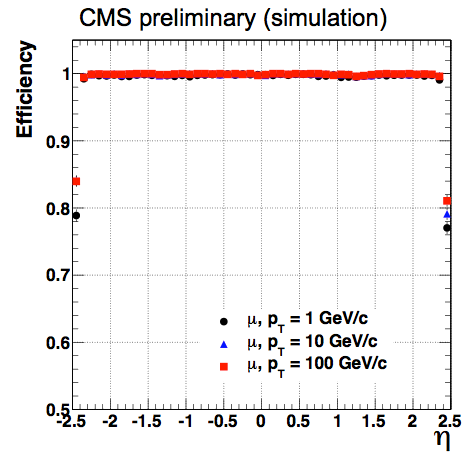
\includegraphics[width=0.45\textwidth]{figures/eff_muon_vs_eta.png} 
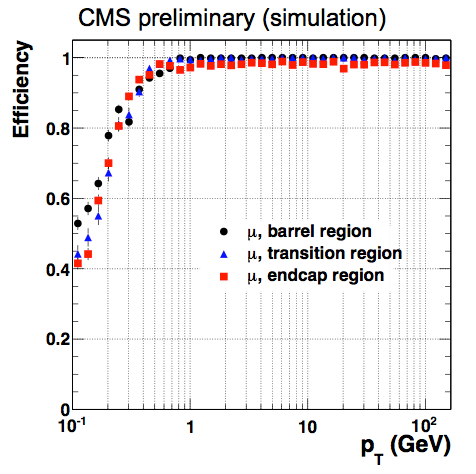
\includegraphics[width=0.45\textwidth]{figures/eff_muon_vs_pt.png} \\
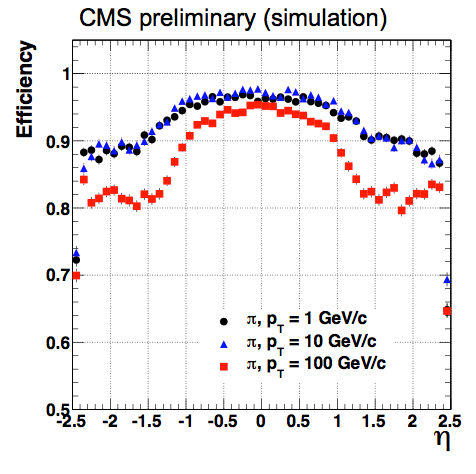
\includegraphics[width=0.45\textwidth]{figures/eff_pion_vs_eta.png} 
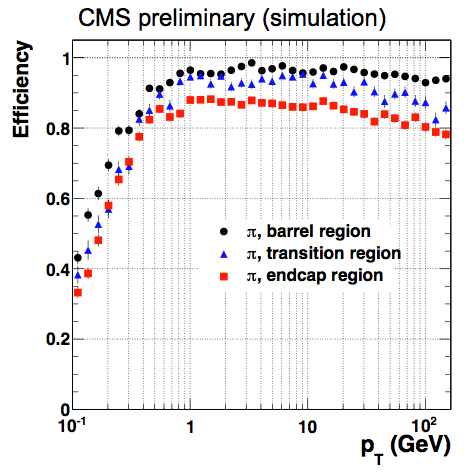
\includegraphics[width=0.45\textwidth]{figures/eff_pion_vs_pt.png} 
\end{tabular}
%https://twiki.cern.ch/twiki/bin/view/CMSPublic/PhysicsResultsTRK
\caption{Tracking efficiency measured using single pion and single muon simulation~\cite{}. 
Top left plot shows the efficiency of muon track reconstruction as a function of \Eta\
for muon \pt\ = 1, 10 and 100~\GeV. 
Top right plot shows the efficiency of muon track reconstruction as a function of \pt\
for different \Eta\ regions. 
Bottom left plot shows the efficiency of pion track reconstruction as a function of \Eta\
for pion \pt\ = 1, 10 and 100~\GeV. 
Bottom right plot shows the efficiency of pion track reconstruction as a function of \pt\
for different \Eta\ regions. 
These plots show that the tracking efficiency for muons is very close to 100~\% 
in the region of phase space we are interested in for this analysis
($\pt>10~\GeV$ and $|\Eta|<2.4$). Efficiency for pion is lower than the one for muon 
because pions decay in flight($\pi^+\to\mu^+\nu_\mu$).  
% pi+ -> mu+ nu_mu (~ 100%, ctau = 7.8 m) 
% simple calculation : e^{-1/7.8} = 0.88 
% about 12% of pions decay in the tracker
} 
\label{fig:TrackingEffMC} 
\end{figure} 

\begin{figure}[htp] 
\centering 
\begin{tabular}{c} 
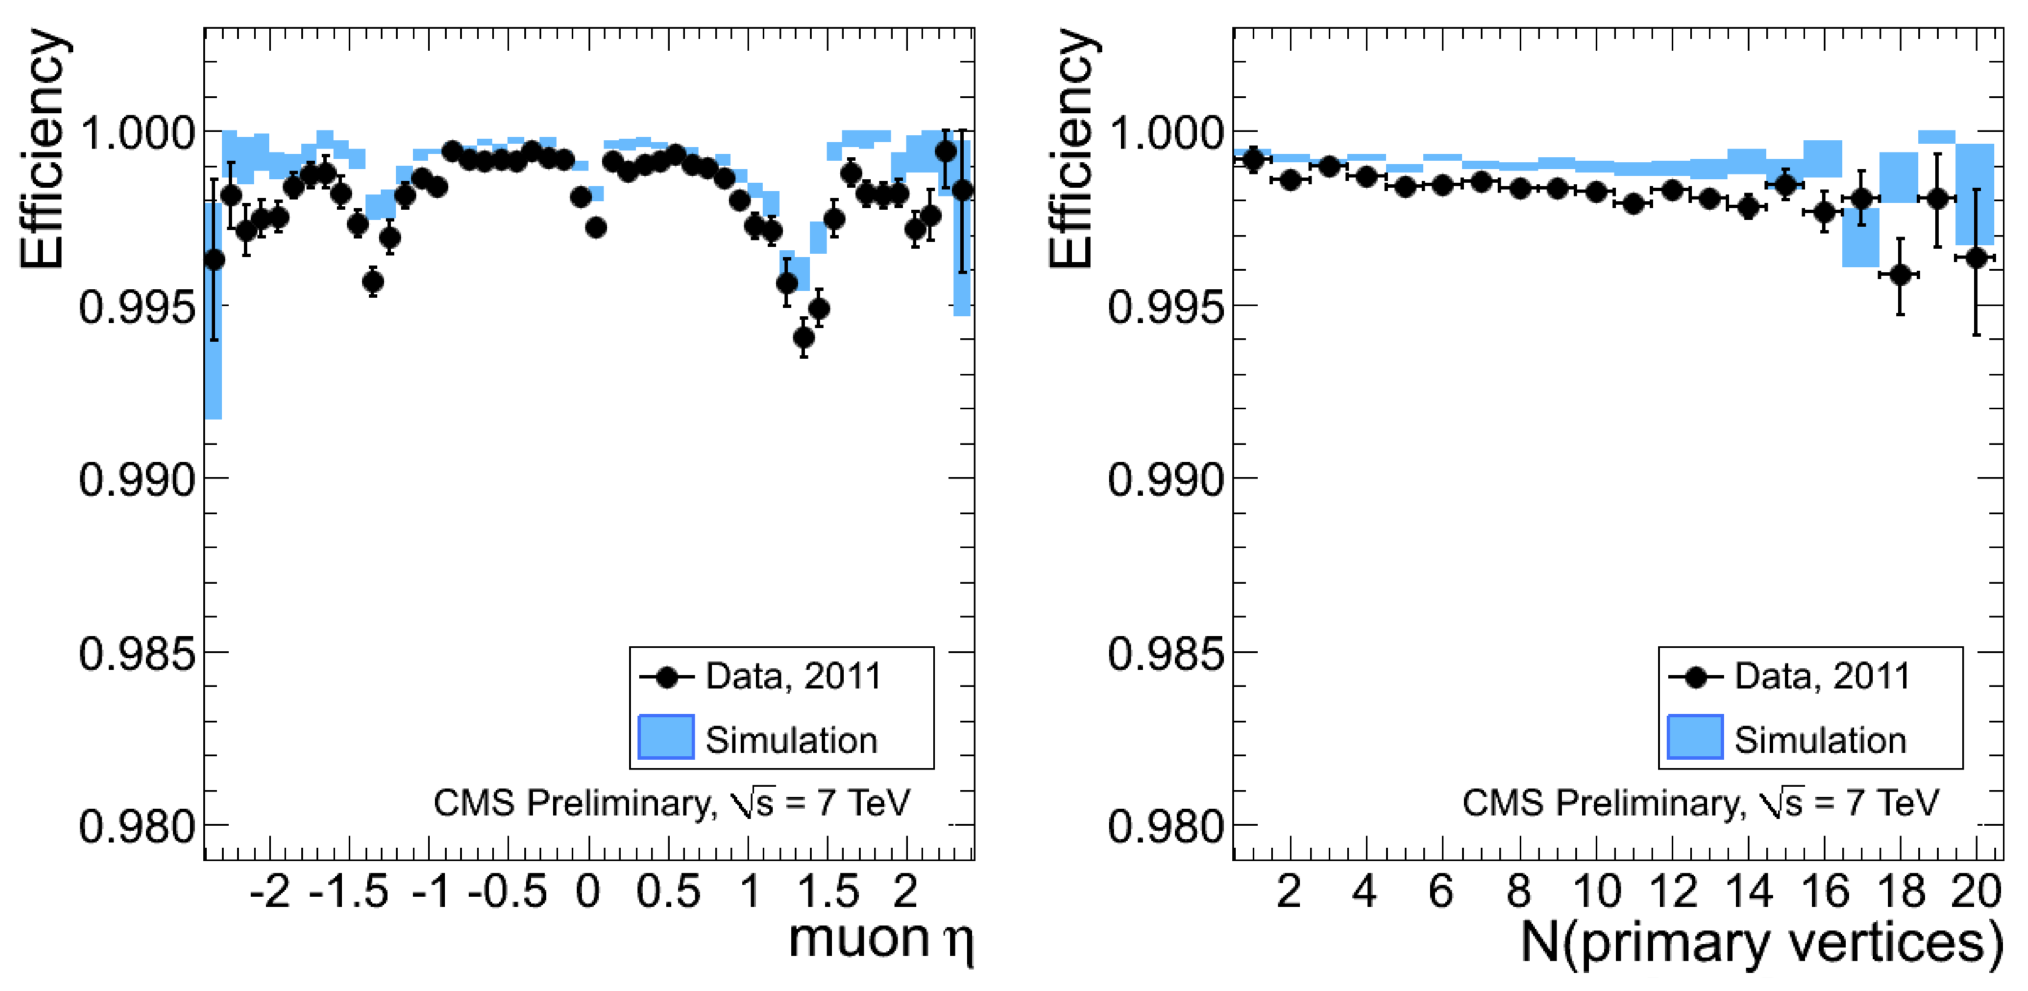
\includegraphics[width=0.9\textwidth]{figures/MuonTagAndProbeEfficiency.png} 
\end{tabular} 
\caption{Muon tracking efficiency in data and MC as a function of 
\Eta(left) and number of reconstructed vertices(right). The agreement 
between data and MC is at the level of a few permille.} 
\label{fig:TrackingEffData} 
\end{figure} 



\textcolor{blue}{ 
Using the obtained seeds, Kalman filter \cite{} is used to find tracks. 
The Kalman filter generates a tree of track candidates ... 
Staring from innermost strip layer, the filter continues all the way to the 
outermost layer ... \textcolor{red}{fill me}.
At each step of track finding, the track state vector, 
the momementum, direction, position of at the given surface, is carried 
with covaricance matrix to the state vector. 
The filter is composed of propagation and update steps which proceed 
alternatively at each layer. In the propagation step, the track state 
at the current surface is propagated to the next surface with the covariace 
matrix which used linear error propagation. The covariance matrix includes 
the effects of materials that the track should cross to reach the next surface. 
The effects of Multiple Coulomb scattering as well as \brem\ for electrons 
are added to the covariance matrix. The momemtum is subtacted by the mean of energy 
loss and the variance of the energy loss distribution is added to the the variance 
of momentum.  In the update step, the propagated state from the previous surface 
is combined with the measurement of the currect surface. 
}


%%%%%%%%%%%%%%%%%%%%%%%%%%%%%%%%%%%%%%%%%%%%%%%%%%%%%%%%%%%%%%%%%%
\section{ Event Primary Vertex }
\begin{itemize}
\item \textcolor{red}{Vertex reconstruction : vertex finding, vertex fitting, ...}
\end{itemize}


The primary vertex, the space point where an interaction takes place,
is reconstructed using reconstructed tracks decribed in the previous section. 
The tracks are selected based on the compatibility with interaction 
region(transverse impact parameter significance with respect to the beamline be less than 5), 
number of hits in the tracker(more than 4(2) hits in silicon strips(pixel detector)) 
and the track fit quality($\chi^2/\textrm{ndof}$ less than 20).
The selected tracks are clustered using Deterministic Annealing algorithm~\cite{DAclustering}.
Only is used the z information at the point of the closest approach(PCA) with 
respect to the beem line. 
% look at http://cmssw.cvs.cern.ch/cgi-bin/cmssw.cgi/CMSSW/RecoVertex/PrimaryVertexProducer/python/OfflinePrimaryVerticesDA_cfi.py?revision=1.8&view=markup
% It says : distance of closest approach < 5sig, #hits >=5(2) for silicon(pixel), chi2/ndf < 5
Then, an adaptive vertex fit~\cite{AdaptiveVertexFit} is performed using the clustered tracks 
for each primary vertex
which has at least two associated tracks. The fit calculates the best estimates 
of the vertex parameters such as position and covariant matrices. 
The vertex is retained if the distance between the vertex and the beam line 
is less than 1~\cm.
%In case there is less than two tracks beam spot is used as a primary vertex. 

Fig.~\ref{fig:VtxEff} shows the vertex reconstruction efficiency as a function 
of number of tracks($N_{track}$) for data and simulation, 
and the transverse(X) and longitudinal vertex resolution 
as a function of $N_{track}$ for jet-enriched data and min-bias data. 
%https://twiki.cern.ch/twiki/pub/CMSPublic/PhysicsResultsTRK/20120911_TRKPOG_Plots_Vertex2012.pdf
The recontruction efficiency is very close to 100~\% with  
$N_{track}>2$. The transverse and londitudinal resolutions measured with 
min-bias data are less than 
30 and 40~\um, repectively, with $N_{track}=30$.

\textcolor{red}{what is the average 
number of tracks for HWW events? want to read off the efficiency from the plots. 
Calculate number of tracks associated with the event PV.}

\begin{figure}[htp] 
\centering 
\begin{tabular}{c} 
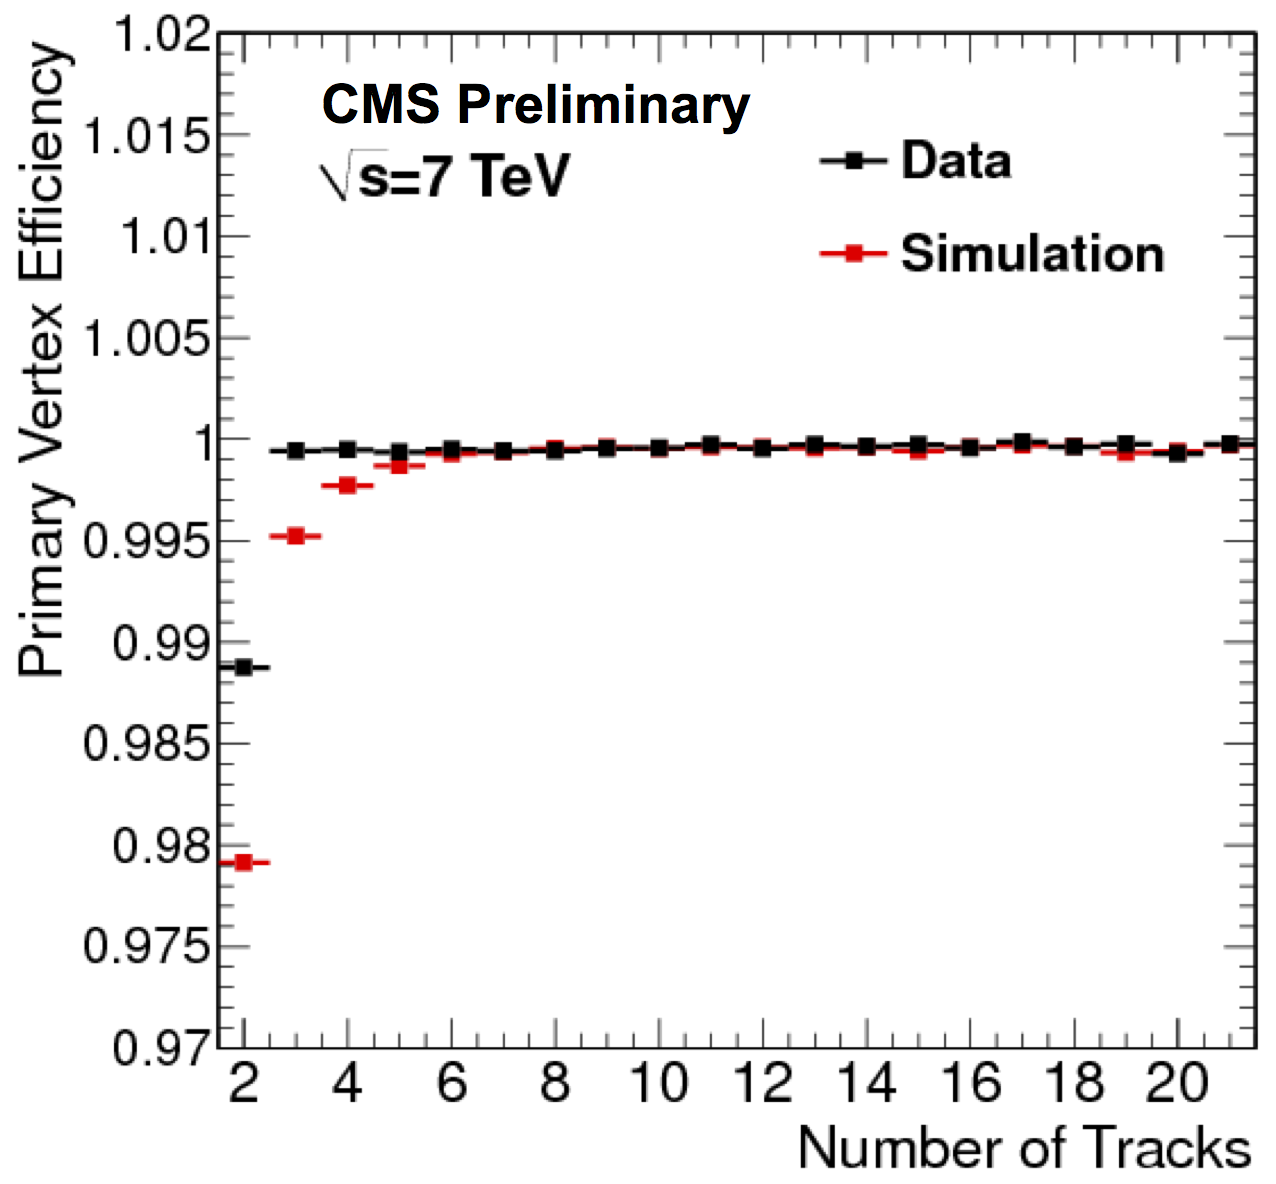
\includegraphics[width=0.45\textwidth]{figures/PrimaryVertexTagAndProbeEfficiency.png} \\ 
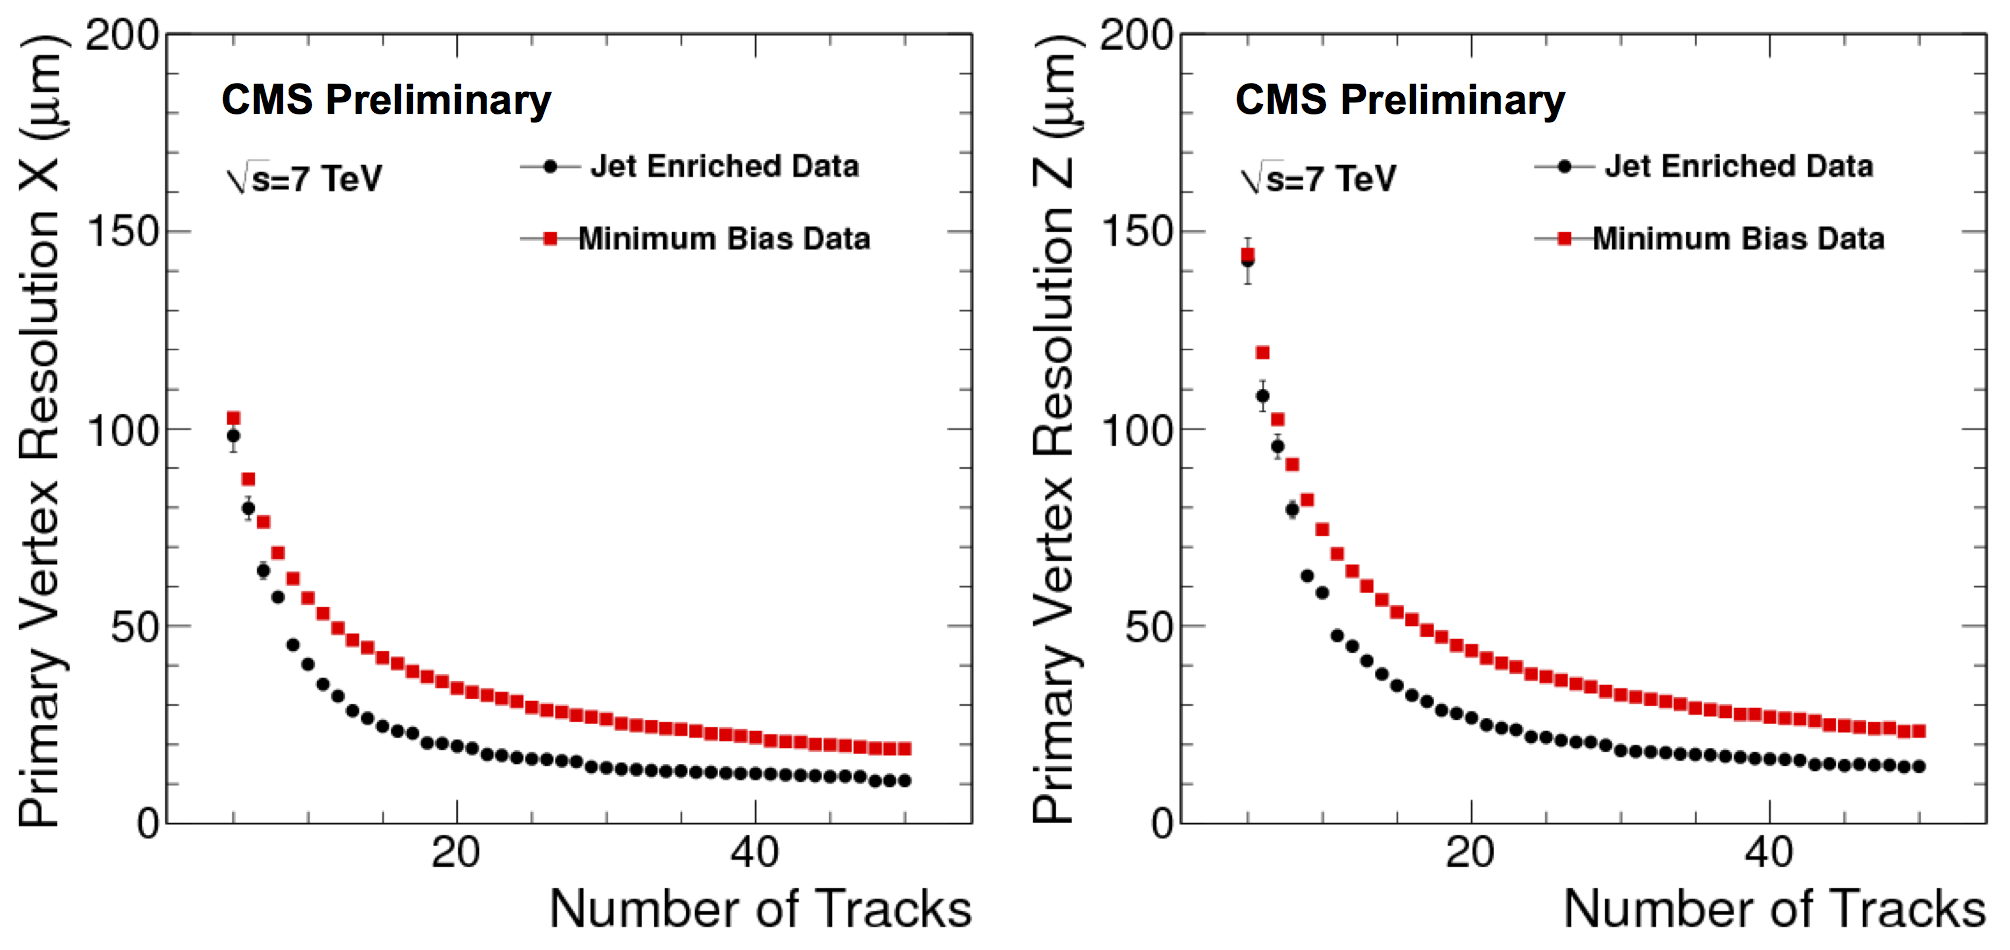
\includegraphics[width=0.9\textwidth]{figures/PrimaryVertexResolutions.png}  
\end{tabular} 
\caption{Vertex resolution in X and Z as a function of associated tracks
for data and Simulation at the top. 
Vertex reconstuction efficiency as a function of number of associated tracks
for jet-enriched data and min-bias data at the bottom. }
\label{fig:VtxEff} 
\end{figure} 

%%%%%%%%%%%%%%%%%%%%%%%%%%%%%%%%%%%%%%%%%%%%%%%%%%%%%%%%%%%%%%%%%%
\section{ Electron }

\textcolor{red}{How is the location of electron calculated !!}

Electrons are reconstructed using information from tracker and ECAL 
as an electron leaves hits in the tracker and makes energy deposit in ECAL.
To reconstruct an electron, ECAL clustering is done first to collect energy 
spread including \brem\ which is called ''supercluster", 
and the track reconstrunction performed using a pixel seed found 
by supercluster-driven method~\cite{Baffioni:2006cd}.  
 
The electrons form electromagnetic shower and make their energy deposit in ECAL. 
A test beam result shows that for a single electron in barrel of an energy 120~\GeV, 
97 \%  of its energy is stored in a $5\times5$ crystal cluster~\cite{Baffioni:2006cd}. 
But, when an electron travels in the tracker which is in a strong magnetic field, 
it radiates photons by \brem\ and the energy deposit 
in the ECAL has a spread in $\phi$. The size of the energy loss in the tracker 
is very significant enough to be included for electron energy calculation. 
For example, for elecrrons of energy 10, 30, 50~\GeV, about 35 \% of electrons 
lose more than 70 \% of their initial energy via \brem\ and about 10 \% of them 
loss more than 95 \%~\cite{Baffioni:2006cd}. Therefore, in order to 
obtain the initial electron energy, it is critical to collect all \brem\ photons.
The algorithm for this purpose is called super-clustering algorithm~\cite{Baffioni:2006cd}.

CMS employs two algorithms, hybrid for barrel region and island for endcap region. 
The hybrid algorithm first forms a domino of 3 or 5 crytals in \Eta, and
dynamically searches for dominos in $\phi$ separated by a domino with energy less 
than a cerntain threshold (100~\MeV).
The island algorithm starts with making a cluster from a seed crystal with energy deposit 
above a cerntain threshold, and collect crystals around it in $\phi$ first and then $\eta$ direction. 
The resultant clusters in narrow $\eta$-window and wider $\phi$-window 
are then used to construct a supercluster.

Once the energy is collected, electron tracks are reconstructed. The first step is 
to generate seeds to start the tracking algorithm. The energy-weighted mean 
supercluster position is extrapolated to the interaction point(beam spot) 
to find compatible hit in the pixel detector assuming both charge hypotheses. 
The innermost layer is looked for first with loose $\Delta\phi$ and $\Delta z$ window. 
If compatible hits are not found in the first layer, search goes on to the next layer. 
If a compatible hit is found, the z coordiate of the primary vertex is calculated 
and the predicted trajectory is used to find compatible hit(s) in the next pixel layer(s).  
Using the selected seed, compatible hits in the next silicon layer are looked for  
and extrapolation is done to the next layer using Beath-Heitler modeling of electron 
\brem~\cite{BetheHeitler} 
and Gaussian Sum Filter(GSF) \cite{0954-3899-31-9-N01} which assumes that the pdf of 
Bethe-Heitler model is a Gaussian mixture. 
%The Beath-Heitler modeling is ...  
%The GSF is ... 
The procedure is continued to the last layer unless two consecutive hits are not found. 
At each layer, trajectory state is updated using weighed mean of measurements 
and prediction. In case of multiple compatible hits, the two most compatible ones 
from $\chi^2$ test are kept. Finally, a track is created if there are at least five hits. 

An electron candidate is reconstructed if there is a track and a supercluster energy deposit
compatible with the track momentum. 

\textcolor{red}{want to talk about fakes here?} 
When there is a random combination of 
a track from $\pi^\pm$ and a supercluster energy deposit from $\pi^0$ that eventually 
decays to two photons, a fake electron candidate can be made. 
In order to suppress them, we apply electron selection which is composed of 
requirements on identification(track-to-supercluster matching, 
track fit quality, shower shape, energy loss due to \brem\, ratio of hadronic energy
to electromagnetic energy), isolation, impact parameter.  
Other source of fake electrons is a photon conversion to a pair of electron and a positron 
in the material. If the conversion is asymmetric, \textit{i.e.} one particle carries 
most of the photon momentum, that particle can be selected as an electron 
candidate. Thus, we apply additional requirement on the convertion rejection.

Fig.~\ref{fig:ElectronEnergyResMC} shows the resolution of reconstructed electron energy 
as a function of the true electron energy measured with simulation~\cite{PAS-HIG-13-002}.   
As shown in the figure, precision is dominated by information from tracker(blue reverse 
trianle) and ECAL(green upright triangle) at low and high energy, respectively. 
The final resolution comes from the combination of the two information weighted by 
their errors(red star). These errors are evaluated by the half minimum width that 
contains 68.3\%(Gaussian 1$\sigma$ width) in the energy distribution. 
The red circle corresponds to the width of Guassian fit of the core of the 
energy distribution. 

\begin{figure}[htp] 
\centering 
\begin{tabular}{c} 
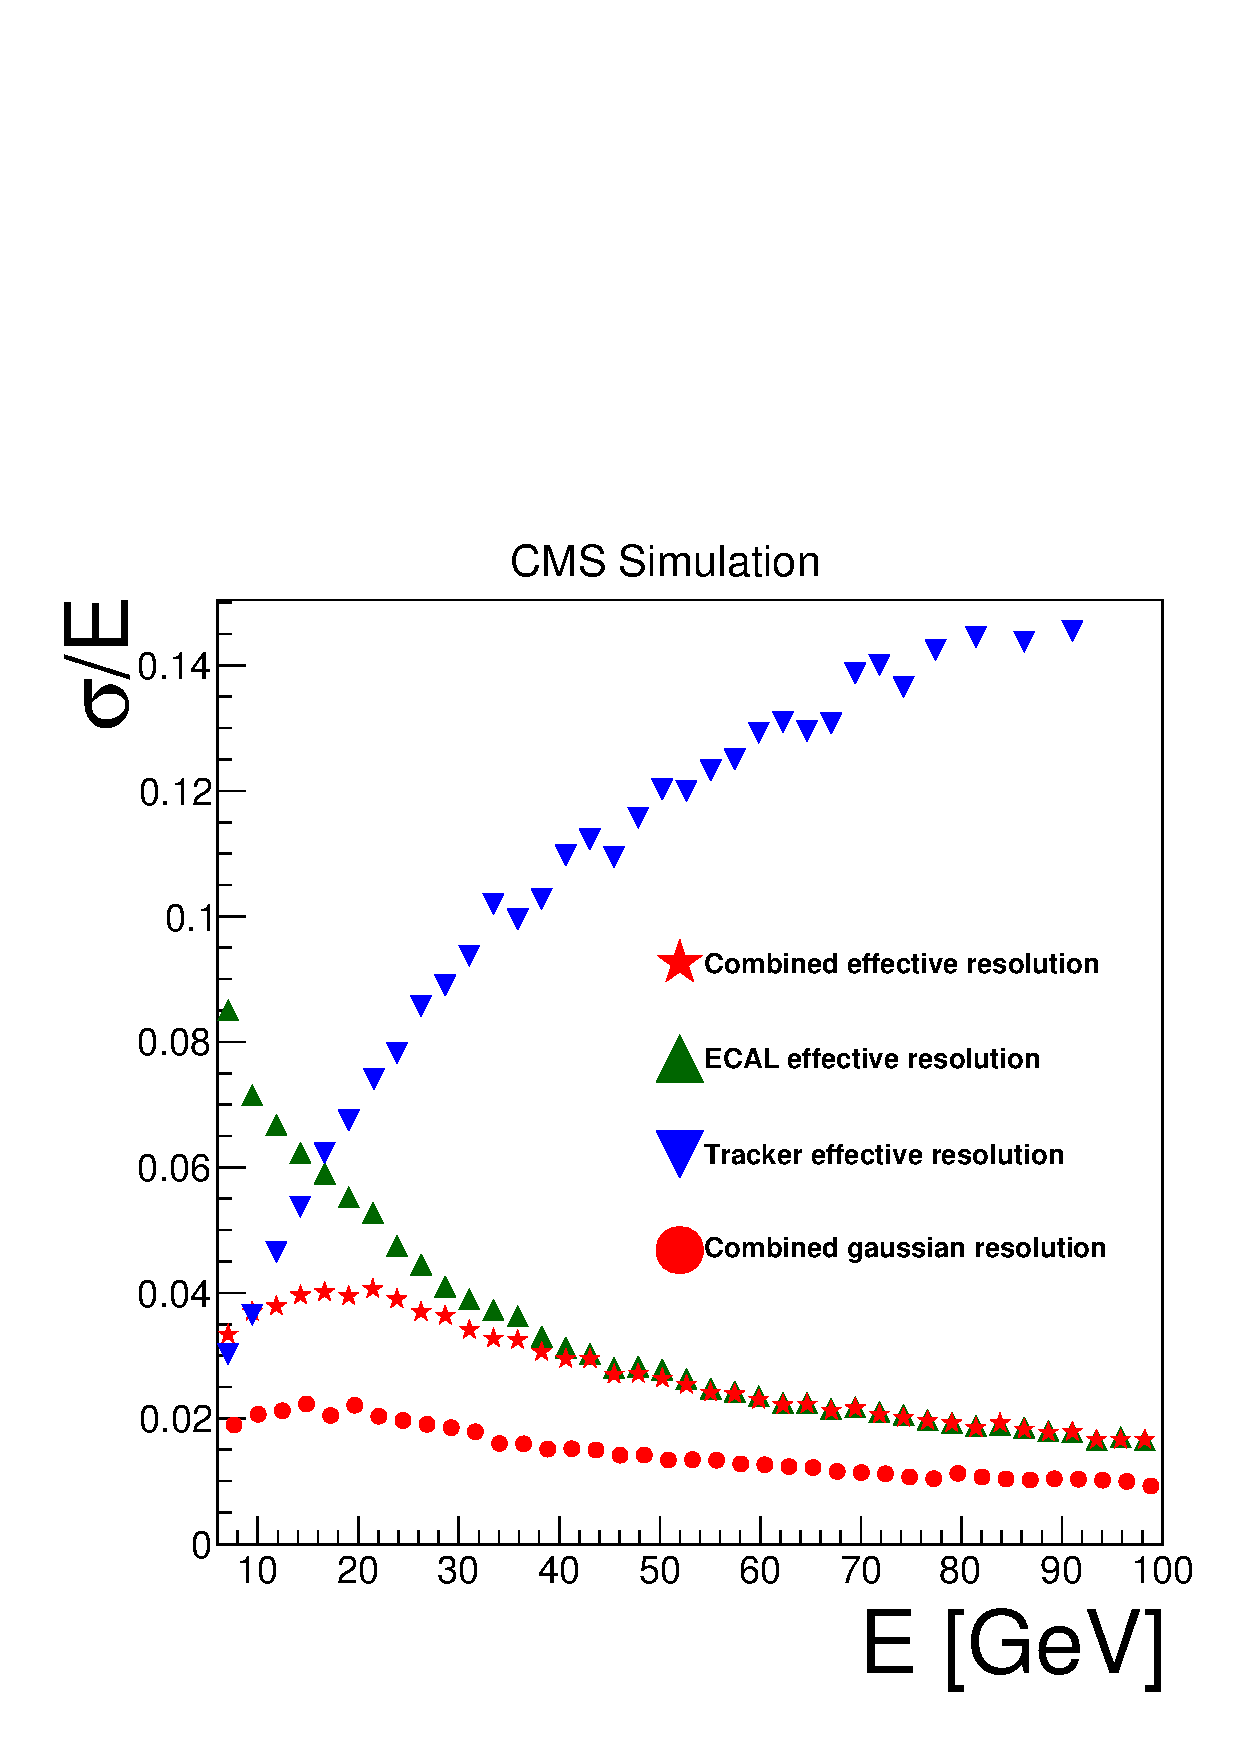
\includegraphics[width=0.6\textwidth]{figures/effRMSfinal-3.pdf} 
\end{tabular} 
\caption{Energy resolution of reconstructed electrons as a function 
of generated electron energy from different information 
in simulation~\cite{PAS-HIG-13-002}. 
Blue reverse triangle is measured using only tracker information 
and green upright triangle is measured using only ECAL information. 
The red star is a combination of the tracker and ECAL measurments. 
The resolution is estimated the half minimum width that
contains 68.3\%(Gaussian 1$\sigma$ width) in the energy distribution
as denoted as effective resolution. The red circle corresponds to the 
width of Guassian fit of the core of theenergy distribution.
}
\label{fig:ElectronEnergyResMC} 
\end{figure} 

%%%%%%%%%%%%%%%%%%%%%%%%%%%%%%%%%%%%%%%%%%%%%%%%%%%%%%%%%%%%%%%%%%
\section{ Muon }

In CMS there are three types of muon reconstruction approaches 
depending on the information(detectors) used in the reconstruction~\cite{cmstdr1}.  

The \textit{Standalone} muon reconstruction uses information from 
the muon system(DT, CSC, RPC), \textit{i.e.} the inner tracker information is not used. 
It starts with the reconstruction of the track segments in the muon chambers. 
The digitized electronic signals in DT, CSC, and RPC are used to 
reconstruct hits. Then, the hits in DT and CSC are matched to form the segments. 
The information of these segments, such as momentum, at the innermost 
muon chamber is used as a seed to construct a muon track using Kalman-filter 
algorithm. The Kalman-filter is an iterative altorithm 
that updates the track parameters iteratively as it goes to the next station. 
At each step of estimating the track parameters, if no matching segment is found 
then the search continues to the next station taking into account the detector 
effects such as multiple scattering and energy loss in the material. 
The procedure goes until the outermost station updating the track parameters 
at each step. After this, the Kalman-filter is applied from the outermost to 
the innermost station, and the track parameters are defined at the innermost 
station. As the last step, the measured muon track is extaploated to the interaction 
point and a vertex-constrained fit is performed to get the final track parameters. 

The \textit{Tracker} muon reconstruction uses information from  
the inner tracker, \textit{i.e.} the muon system information is not used
for the momentum measurement. This approach considers all tracks as 
potential muon candiates and checks their compatibility with 
muon system. All tracker tracks with $\pt>0.5~\GeV$ and $p>2.5~\GeV$ 
are extrapolated to the muon system considering the expected detector effects 
such as magnetic field, multiple scattering, and energy loss in the material. 
If there is at least one muon segment matched to the 
extrapolated track, this muon is considered as the Tracker muon. 
Tracker muon gives good momentum measurement and identification for low \pt\ muons
which are hard to be reconsructed because they do not leave enough track segments 
in the muon system. 

The \textit{Global} muon reconstruction uses information from both tracker 
and the muon system. For a standalone muon track obtained by the way explained 
already, matching between the muon track and a tracker track is performed. 
The muon track at the innermost station is extrapolated to the last layer 
of the tracker considering the expected detector effects 
such as magnetic field, multiple scattering, and energy loss in the material.
Once the matching is done, the Kalman-filter is used to reconstruct the tracks. 
After that, all reconstructed tracks are fitted again without constraints on the 
beamspot using all hits used to reconstruct standalone muons and the hits 
in the silicon strips. A fit is done again using the tracker hits and the 
hits in the innermost muon station, and the fit quality is compared with 
that of the tracker-only fit. This is to detect muon \brem\  or 
any loss of energy before reaching the muon station.

In summary, there are three approaches for muon reconstruction in CMS. 
Having multiple algorithms provides more reliable muon reconstruction 
and physics analysis can choose their algorithms for their interests. 
\begin{figure}[!hbtp]
\centering
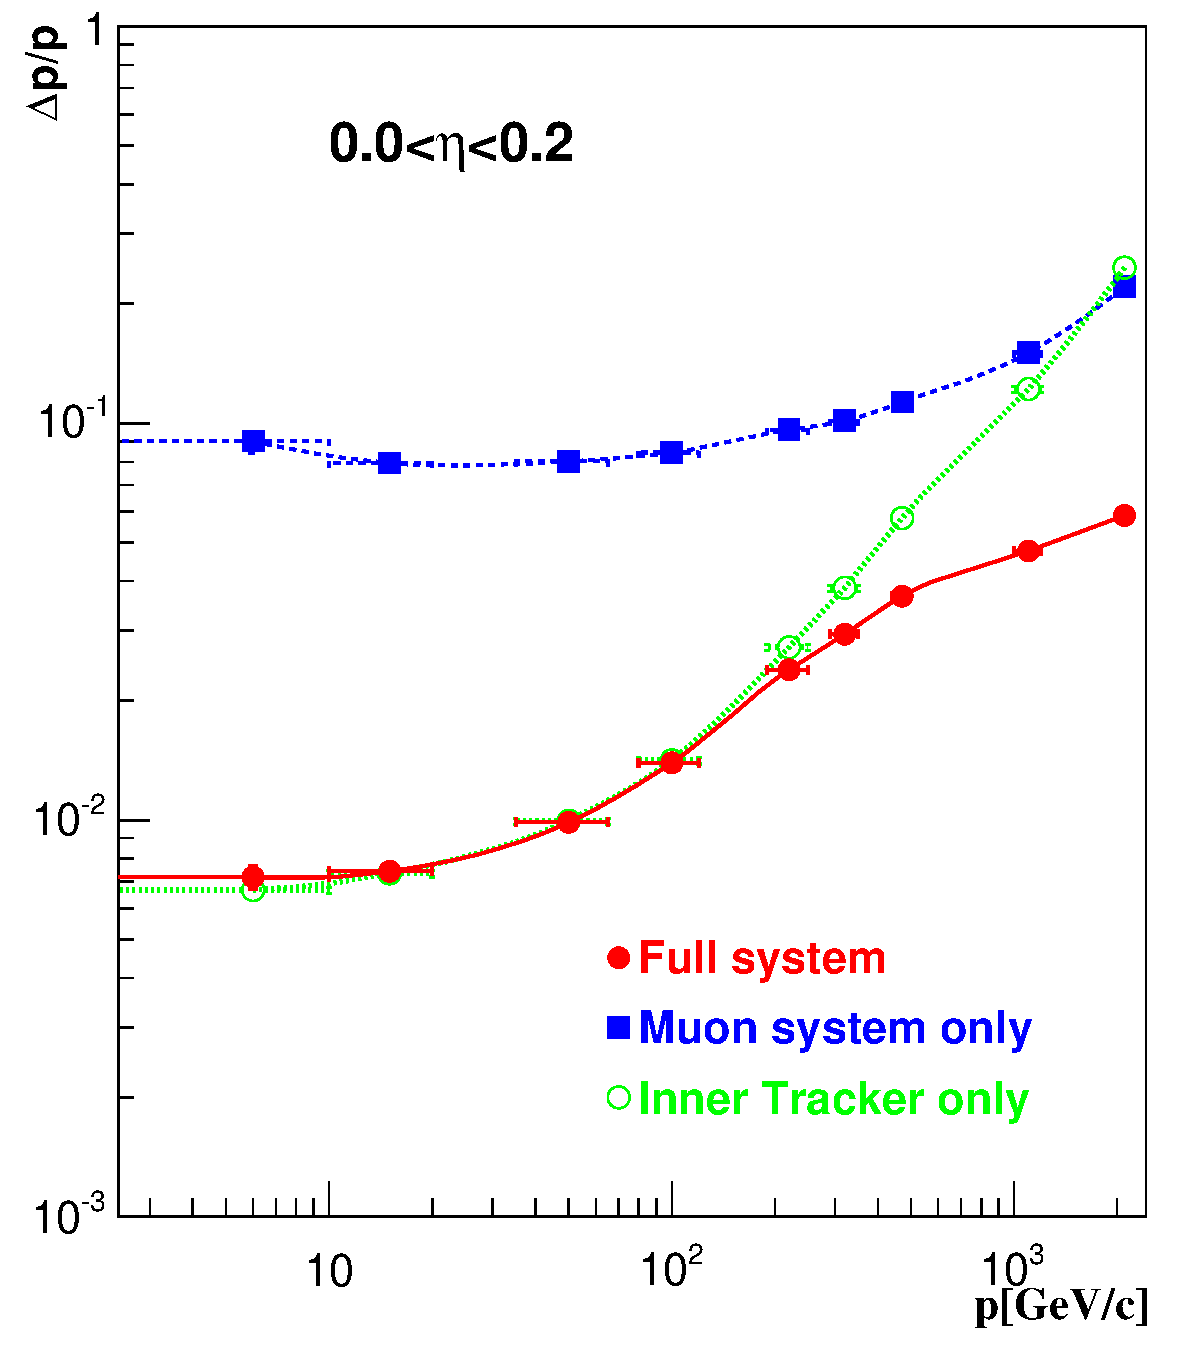
\includegraphics[width=.45\textwidth]{figures/Figure_001-005-a.pdf}
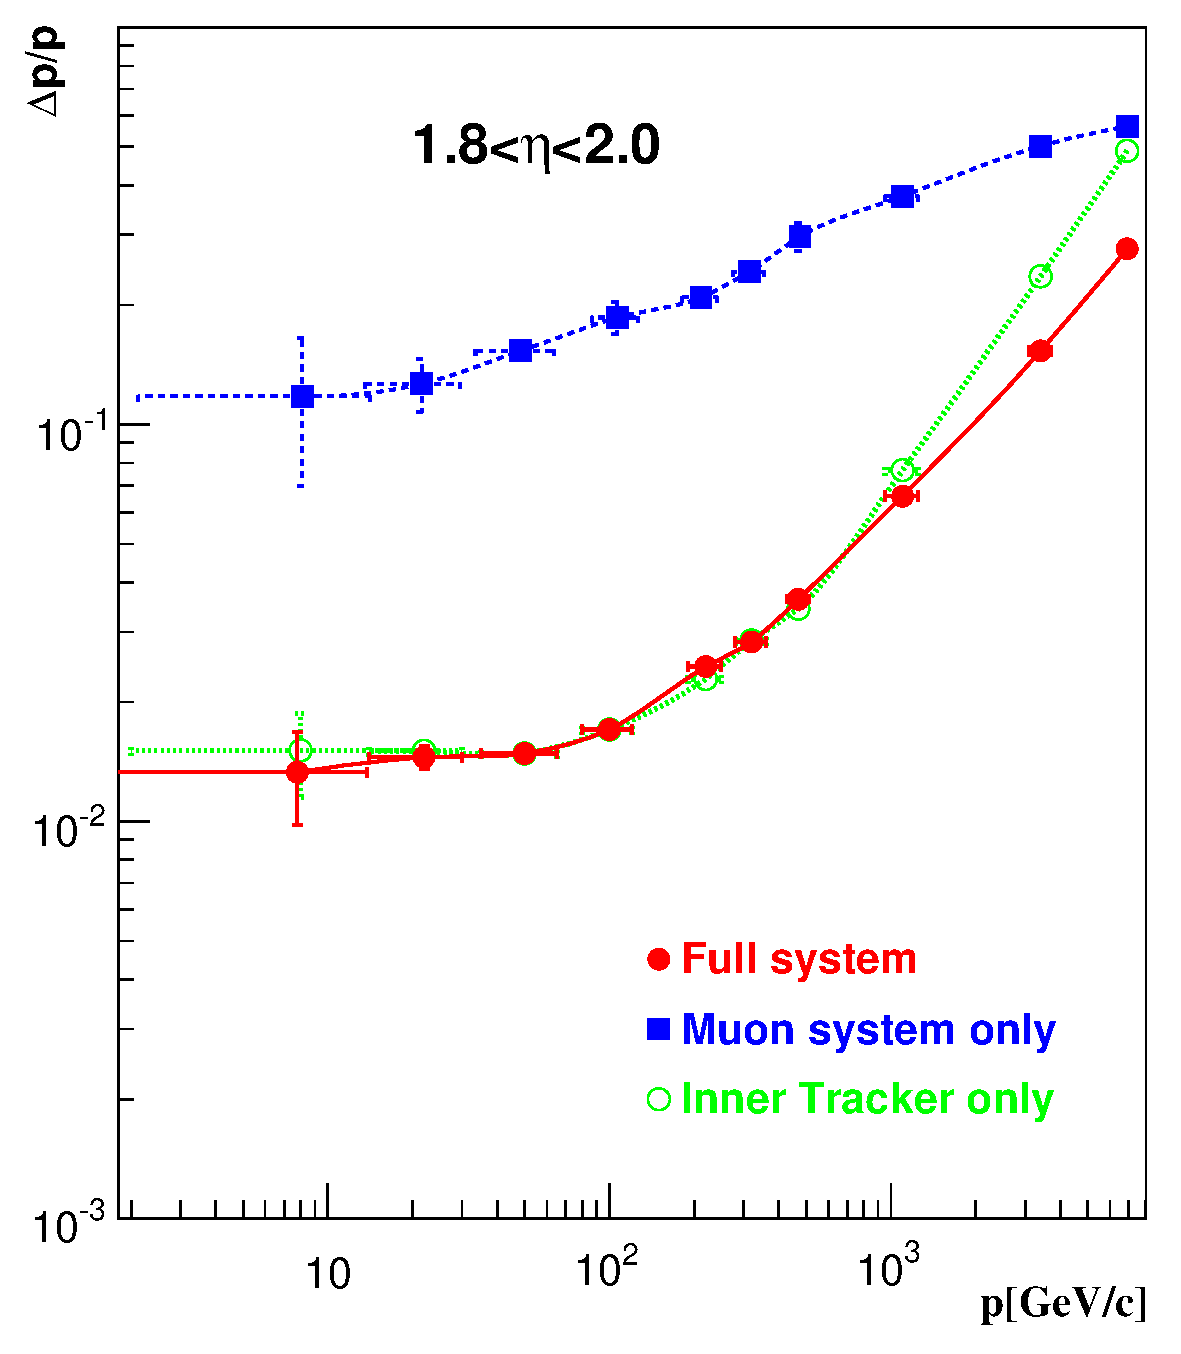
\includegraphics[width=.45\textwidth]{figures/Figure_001-005-b.pdf}
\caption{Resolution of muon momemtun in $0.0<|\eta|<0.2$ and $1.8<|\eta|<2.0$. 
Red, blue and green are global, standalone and tracker muons, respectively.} 
\label{fig:muon_res}
\end{figure}
Fig.~\ref{fig:muon_res} shows the momentum resolution of difference muon 
reconstruction algorithms as a function of muon \pt\ in the barrel(left) and endcap(right). 
The resolution of standalone muons is dominated by mutiple scattering in the material 
before the muon station at $\pt<200~\GeV$ and and by the spacial resolution 
of the muon chambers at $\pt>200~\GeV$. The tracker muons give much better 
resolution at low \pt\, but the resolution goes up to the same level 
with the stanalone muons at very high \pt. 

%%%%%%%%%%%%%%%%%%%%%%%%%%%%%%%%%%%%%%%%%%%%%%%%%%%%%%%%%%%%%%%%%%
\section{ Jet }
\label{sec:jetselection}
\begin{itemize}
\item \textcolor{red}{Jet reconstruction : anti-kT (dR = 0.5) }
\item \textcolor{red}{Jet energy correction : L1Fastjet/L2/L3 (+ Residual correction in data) }
\end{itemize}

%FIXME I am here 
The existence of gluons and quarks in the event is manifested as a hadronic shower, 
``jets", which leaves an energy deposit primarily in the HCAL. 
Thanks to the fine granuality of CMS detector system, individual hadrons can 
be reconstructed by PF algorithm~\cite{}. 
\textcolor{red}{brief explanation on PF algorithm}. 

The jets are reconstructed by clustering individual particles
that come from the same parton. The algorithm works 
such that the two distances are defined, $d_{ij}$ being the 
distance between particle i and j and $d_{iB}$ being the 
distance between particle i and the beam line. If the minimum 
of $d_{ij}$ and $d_{iB}$ is $d_{ij}$ then the two particles are merged,
and if the minimum is $d_{iB}$ then the paritle i is removed from 
the list of paricles because it is thought be a radiation from the beam. 
CMS uses anti-$\textrm{k}_\textrm{T}$ algorithm~\cite{Cacciari:2008gp} 
using PF candiates.  
In this algorithm, the distances are defined as 
\begin{eqnarray} 
d_{ij} 
&=&   
min \left( \frac{1}{k_{Ti}^2}, \frac{1}{k_{Tj}^2} \right) 
\frac{\Delta_{ij}^2}{R^2}, \\ 
d_{iB} 
&=&  
k_{Ti}^{-2}
\end{eqnarray} 
where $k_{Ti}$ is the transverse momentum of particle $i$, 
$\Delta_{ij}^2 = \left( y_i - y_j \right)^2 + \left( \phi_i - \phi_j \right)^2$ 
with $y_i$ and $\phi_i$ being the rapidity and the azimuthal angle of particle $i$,
and $R$ is the scale that determines the distance of the reconstructed jets.   
CMS used $R = 0.5$ for jet resconstruction. 
The clustering uses FastJet algorithm~\ref{Cacciari:2005hq} which
significantly improves the timing of calculation, and provides  
the jet area used for subtraction of contribution from PU. 

Due to the non-linear calorimeter response of CMS detector, 
the measured jet energy can not be translated into the energy of the true parton which 
initiated the jet. CMS employs jet energy correction(JEC) method \cite{} factorized into 
several levels, L1, L2, L3 and residual corrections for data. 
The L1 correction is the PileUp/noise correction, \textit{i.e.} to remove offset energy 
from PileUp and noise. The correction is composed of two sub-correction, 
one from the real jet energy loss due to detector thresholds and 
the other from PileUp. The offset energy in a jet area is measured as a function 
of \Eta\ in the zero-bias and min-bias samples.    
The L2 correction is to make the jet energy response flat in \Eta.  
At a given \Eta\ response is corrected so that the it becomes at the same level 
of the central region, $|\Eta|<1.3$. So, the correction is relative. 
The correction factors are derived from either MC or using data-driven method
(di-jet balance \cite{}).
The L3 correction is to make the jet energy response flat in \pt.  
The central region, $|\Eta|<1.3$, is used as a referece for the correction. 
Apart from the L2 correction, L3 correction is an absolute correction 
such that the corrected jet \pt\ is same as the \pt\ of the parton that 
initiated the jet. The correction factors are derived from either MC 
or using data-driven method($Z/\gamma^*$+jet balance \cite{}). 
For L2 and L3 corrections, the corrections based on MC truth is done for MC 
and residual corrections are applied to data to account for the small differences 
between data and MC. 

%%%%%%%%%%%%%%%%%%%%%%%%%%%%%%%%%%%%%%%%%%%%%%%%%%%%%%%%%%%%%%%%%%
\section{ Missing Transverse Energy }
\begin{itemize}
\item \textcolor{red}{How MET(pfMET and trackMET) is calculated } 
\item \textcolor{red}{mention MET $\phi$ modulation correction }
\item \textcolor{red}{define projected MET (compare signal and bkgd, (ex) \ztt)}
\item \textcolor{red}{cut values ($\textrm{minMET} > 20~\GeV$) }
\end{itemize}
There are some particles that do not interact with materials. One of them is neutrino.
When neutrinos are produced at the collider, they do not leave any signature 
in the detector, so they can not be reconstructed. However, we can infer 
the existence of neutrino, or any weakly-interacting particles, by computing 
the imbalance in the vector sum of transverse momenta of the reconstructed particles.
The transverse momentum of the initial particles is zero 
\footnote{It is not perfectly zero because partons have transverse movements 
inside the proton. But, the energy of their motion is at most a few hundred \MeV\
which is much less than the resolution of measurements.}.
By momentum convervation, the total momentum of the particles produced 
after collision should be 0 as well. 
So, if the transverse momenta of all particles in the final state are summed up, 
the negative value of the vector sum should correspond to the transverse momentum 
sum of neutrinos. Thus, we define ``Missing Transverse Energy(\met)", 
\begin{eqnarray} 
\overrightarrow{\met} = - \sum^{\textrm{All PF candidates}}_i \overrightarrow{\pt}(i).
\end{eqnarray} 
In this analysis, \met\ is calculated with particles reconstructed using PF algorithm~\cite{}.

The $\phi$ distribution of true \met\ should be flat because of the rotational 
symmetry of collisions with respect to the beam axis. However, possibly due to 
anisotropic detector response, inactive calorimeter response, detector misalignments, 
and displacement of the beam spot, the $\phi$ distributions of \met\ in both 
MC and data are not flat, but a sinusoidal shape with a period $2\pi$. 
Thus, we correct this by shifting the origin of the coordinates 
in the transverse momentum plane for x and y components individually. 
Since the size of the shift increases 
linearly as a function of number of reconstructed primary vertices, 
the form of correction is given by 
\begin{eqnarray} 
\alpha + \beta N_{\textrm{vertex}}
\end{eqnarray} 
where $\alpha$ and $\beta$ shown in Table~\ref{tab:metxycorrection} are constants 
and $N_{\textrm{vertex}}$ is the number of primary vertices. 
\begin{table}[htp] 
\begin{center} 
\begin{tabular}{c||c|c|c} 
\hline 
                       &                  & $\alpha$ &  $\beta$  \\
\hline \hline 
\multirow{2}{*}{MC}    & correction for X & $-3.00 \times 10^{-2}$ & $-6.62\times 10^{-2}$  \\
                       & correction for Y & $3.71\times 10^{-1}$   & $-1.49\times 10^{-1}$  \\
\hline 
\multirow{2}{*}{Data}  & correction for X & $3.54\times 10^{-1}$   & $2.65\times 10^{-1}$   \\
                       & correction for Y & $1.89\times 10^{-1}$   & $1.66\times 10^{-1}$   \\
\hline 
%    metx -= (+3.54233e-01 + 2.65299e-01*nvtx_);
%    mety -= (+1.88923e-01 - 1.66425e-01*nvtx_);
%    metx -= (-2.99576e-02 - 6.61932e-02*nvtx_);
%    mety -= (+3.70819e-01 - 1.48617e-01*nvtx_);
\end{tabular} 
\caption{Parameters used for XY shift correction for \met.} 
\label{tab:metxycorrection} 
\end{center} 
\end{table} 
\textcolor{red}{optional : show the met distribution before/after the correction}

The performance of met reconstruction is severely degraded in high luminosity environment 
because of random contribution of paricles from PileUp to the \met\ calculation. 
So, we use another definition of \met\ which is calculated with only charged 
PF candidates associated with the event primary vertex. Since particles from 
other vertices that the event primary vertex are excluded in the \met\ calculation,
the \met\ calculated using this method is independent of number of PileUps.  
This \met\ definition is called ``\trkmet" and exact definition is
\begin{eqnarray} 
\overrightarrow{\trkmet} 
= 
- \overrightarrow{\pt} (\ell_1)  
- \overrightarrow{\pt} (\ell_2)  
- \sum^{\textrm{All charged PF candidates}}_i \overrightarrow{\pt}(i)
\end{eqnarray} 
where $\overrightarrow{\pt} (\ell_1)$ and $\overrightarrow{\pt} (\ell_2)$
are the transverse momemta of the leptons. The charged PF candidates must 
meet the following requirements.
\begin{itemize}
\item The longitudinal impact parameter of the track matched to the PF candidate 
      with respect to the event primary vertex should be less than 0.1~cm. 
\item $\Delta R$ between the track matched to the PF candidate and the leptons 
      should be larger than 0.1 in order to avoid counting leptons twice. 
\end{itemize}

%%%%%%%%%%%%%%%%%%%%%%%%%%%%%%%%%%%%%%%%%%%%%%%%%%%%%%%%%%%%%%%%%%
\section{ B-tagging }
\begin{itemize}
\item \textcolor{red}{How B-tagging algorithm works and working point
      (TCHEM : Track Counting High Efficiency Medium)}
\item \textcolor{red}{how the discriminating variable is calculated }
\item \textcolor{red}{quote some performance plots }
\item \textcolor{red}{soft-muon tagging requirement }
\end{itemize}

The presence of a bottom quark in the event is manifested by the presence a secondary vertex. 
The bottom quark is hadronized to a B meson($\textrm{B}^0, \textrm{B}^\pm, ...$) and it 
traverses for a measurable distance before decaying into other particles.
Typically, the b-tagging algorithms use information of the impact parameter(IP) of 
charged particles decayed from the B meson or the distance between the primary vertex 
and the secondary vertex. 
\begin{figure}[htp] 
\centering 
\begin{tabular}{c} 
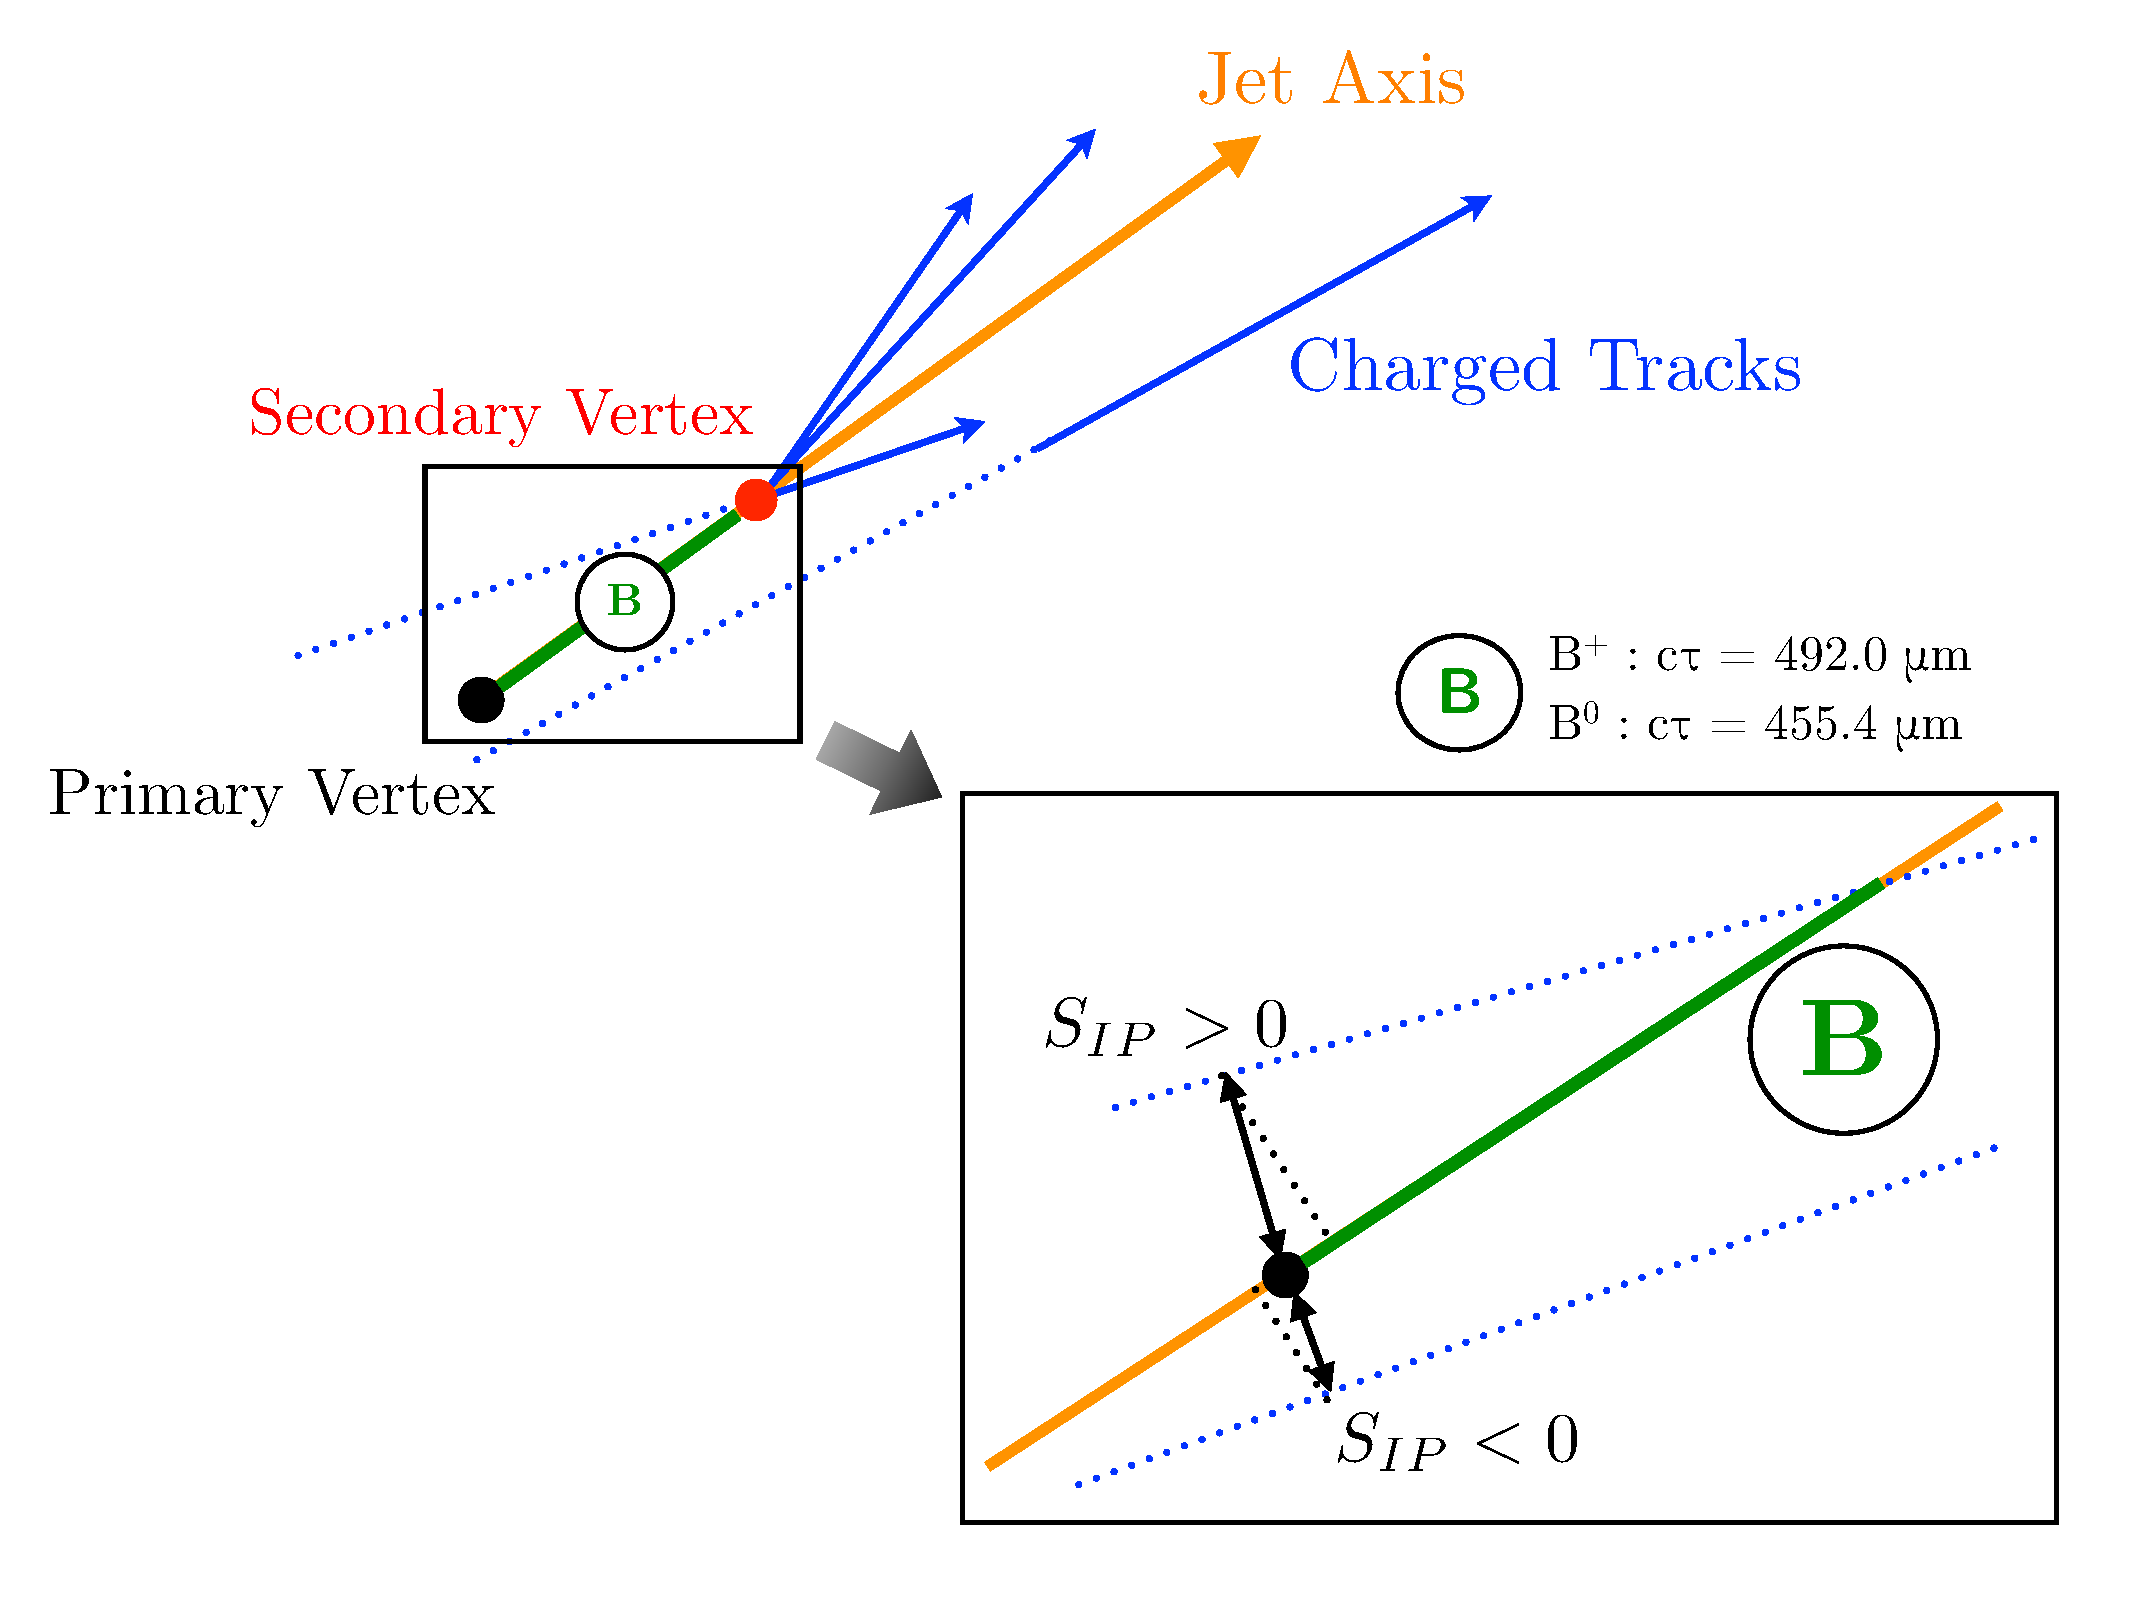
\includegraphics[width=0.99\textwidth]{figures/Btag.pdf} 
\end{tabular} 
\caption{A schematic of b-taging algorithm.}
\label{fig:btag} 
\end{figure} 
The IP is calculated in 3D thanks to the good z resolution of the 
pixel detector. The IP can be signed depending on the position of 
the associated track. The sign is obtained from the sign of the scalar product of 
IP vector from the primary vertex and the direction of the jet the track belongs to
as shown in Fig.~\ref{fig:btag}.
For the decays with sizable lifetime, the IP should be positive in theory, 
but it is not always positive in case the real direction of the B meson 
is different from the direction of the jet. But, they still tend to be positive. 
For the decays with very short lifetiem or random tracks that happen to be 
considered for btagging algorithm, the IP is symmetric around 0.   

In b-tagging algorithm used in this analysis is so called ``TrkCountingHighEff(TCHE)" \cite{}.
This algorithm uses the impact parameter significance, $S_{IP} = IP / \sigma_{IP}$ 
where $\sigma_{IP}$ is the uncertainty of the IP measurement, 
as a discribinating variable. The algorithm requires at least 2 tracks to have $S_{IP}$ 
above a given threshold. Thus, the discriminator is the $S_{IP}$ of the second highest 
significance. 
